\chapter{じぷりについて}

\section{じぷりの概要}%例:レビュー内容
%必要ならここに大見出しの内容
%必要なら下のsubsectionを用いて小見出しをつかう
%\subsection{ここに小見出し}%:発表技法について
本プロジェクトで開発しているHTML5ハイブリッドアプリケーション「じぷり」は、陣川あさひ町会が企画、運営するイベント情報の発信、発信されたイベントへの参加申し込み、雨天延期などの陣川あさひ町会役員による緊急連絡が可能となるアプリケーションである。このアプリケーションの名称は、「陣川」という地域の名称と、「アプリケーション」を組み合わせたものである。本アプリケーションの目標は、陣川あさひ町会のイベント開催に関する問題を解決することを目標設定した。使用場面は新規イベントの開催が決定してから、当日のイベント終了までを想定している。既存の他のアプリケーションと比較した際の優位性として、2点挙げられる。1つ目は、イベント情報を発信する際に、過去のイベント情報からs買う制されたテンプレートを用いることで、次回以降の入力の手間を省くことができる点である。2つ目は、陣川あさひ町会役員にヒアリングを重ねた結果、クライアントが本当に必要とする機能を実装している点である。「じぷり」では対象とするユーザを、町民、町民外、役員に属性分けをした。また、役員については閲覧者と編集者の2つに属性分けをした。「じぷり」では、アプリケーションの初回起動時に、ユーザが町民、町民外、役員のいずれかであるか識別する。その後、役員以外のユーザが利用する「一般モード」か、役員のみが利用する「役員モード」に分類する。次回以降は、この工程は省略する。「一般モード」では、イベント情報とお知らせの閲覧と、イベントへの参加申し込みを可能とした。「役員モード」では、「一般モード」に加えて役員会議など役員以外にとって必要のない情報も含めすべての情報を閲覧できる。次節より「じぷり」の各機能について詳しく記述していく。

\section{イベント管理機能}%例:レビュー内容
\subsection{イベント管理機能の概要}%:発表技法について
イベント管理機能とは「役員モード」の場合のみ利用可能な機能であり、イベント情報の発信と発信した情報の編集、削除することを可能としている。これらは、役員のうち編集者のみが使うことを可能とした。その意図としては、クライアントにヒアリングをした際に、役員の中には上手くアプリケーションを操作出来ないと考えられる方もおり、誤った情報を発信するといったリスクを考えた結果、属性分けをして欲しいという要望を受けたためこの形式を取った。イベント管理機能を実装した意図としては、イベントの情報をFacebookやLINE@など複数のサービスを使用して発信していた従来の方式から、本アプリケーション1つで全てを賄うことを可能とするためである。

\subsection{イベント情報の発信画面}%:発表技法について
イベント一覧リスト画面(図5.1(a))から新規作成ボタンを押すと、イベント情報の発信画面(図5.1(b))に遷移する。イベント情報の発信画面では、入力する情報の属性としてイベント名、日程、場所、開始時間、終了時間、定員、詳細、役員のみに公開の8つに分けた。役員のみに公開とは、役員会議など町民にとっては知る必要のないイベント情報を判別するために設けた。これら8つの属性は、ヒアリングを通して定まったものである。情報を入力した後画面下の作成ボタンを押すことでイベント情報を発信することが可能となる。また、ボタンが押された際に本アプリケーションがインストールされている全ての端末に、イベント情報が発信されたことを伝える通知が行く形式にした。通知機能については、5.6節で詳しく記述する。

\begin{figure}[htbp]
  \begin{center}
    \begin{tabular}{c}

      % 1
      \begin{minipage}{0.33\hsize}
        \begin{center}
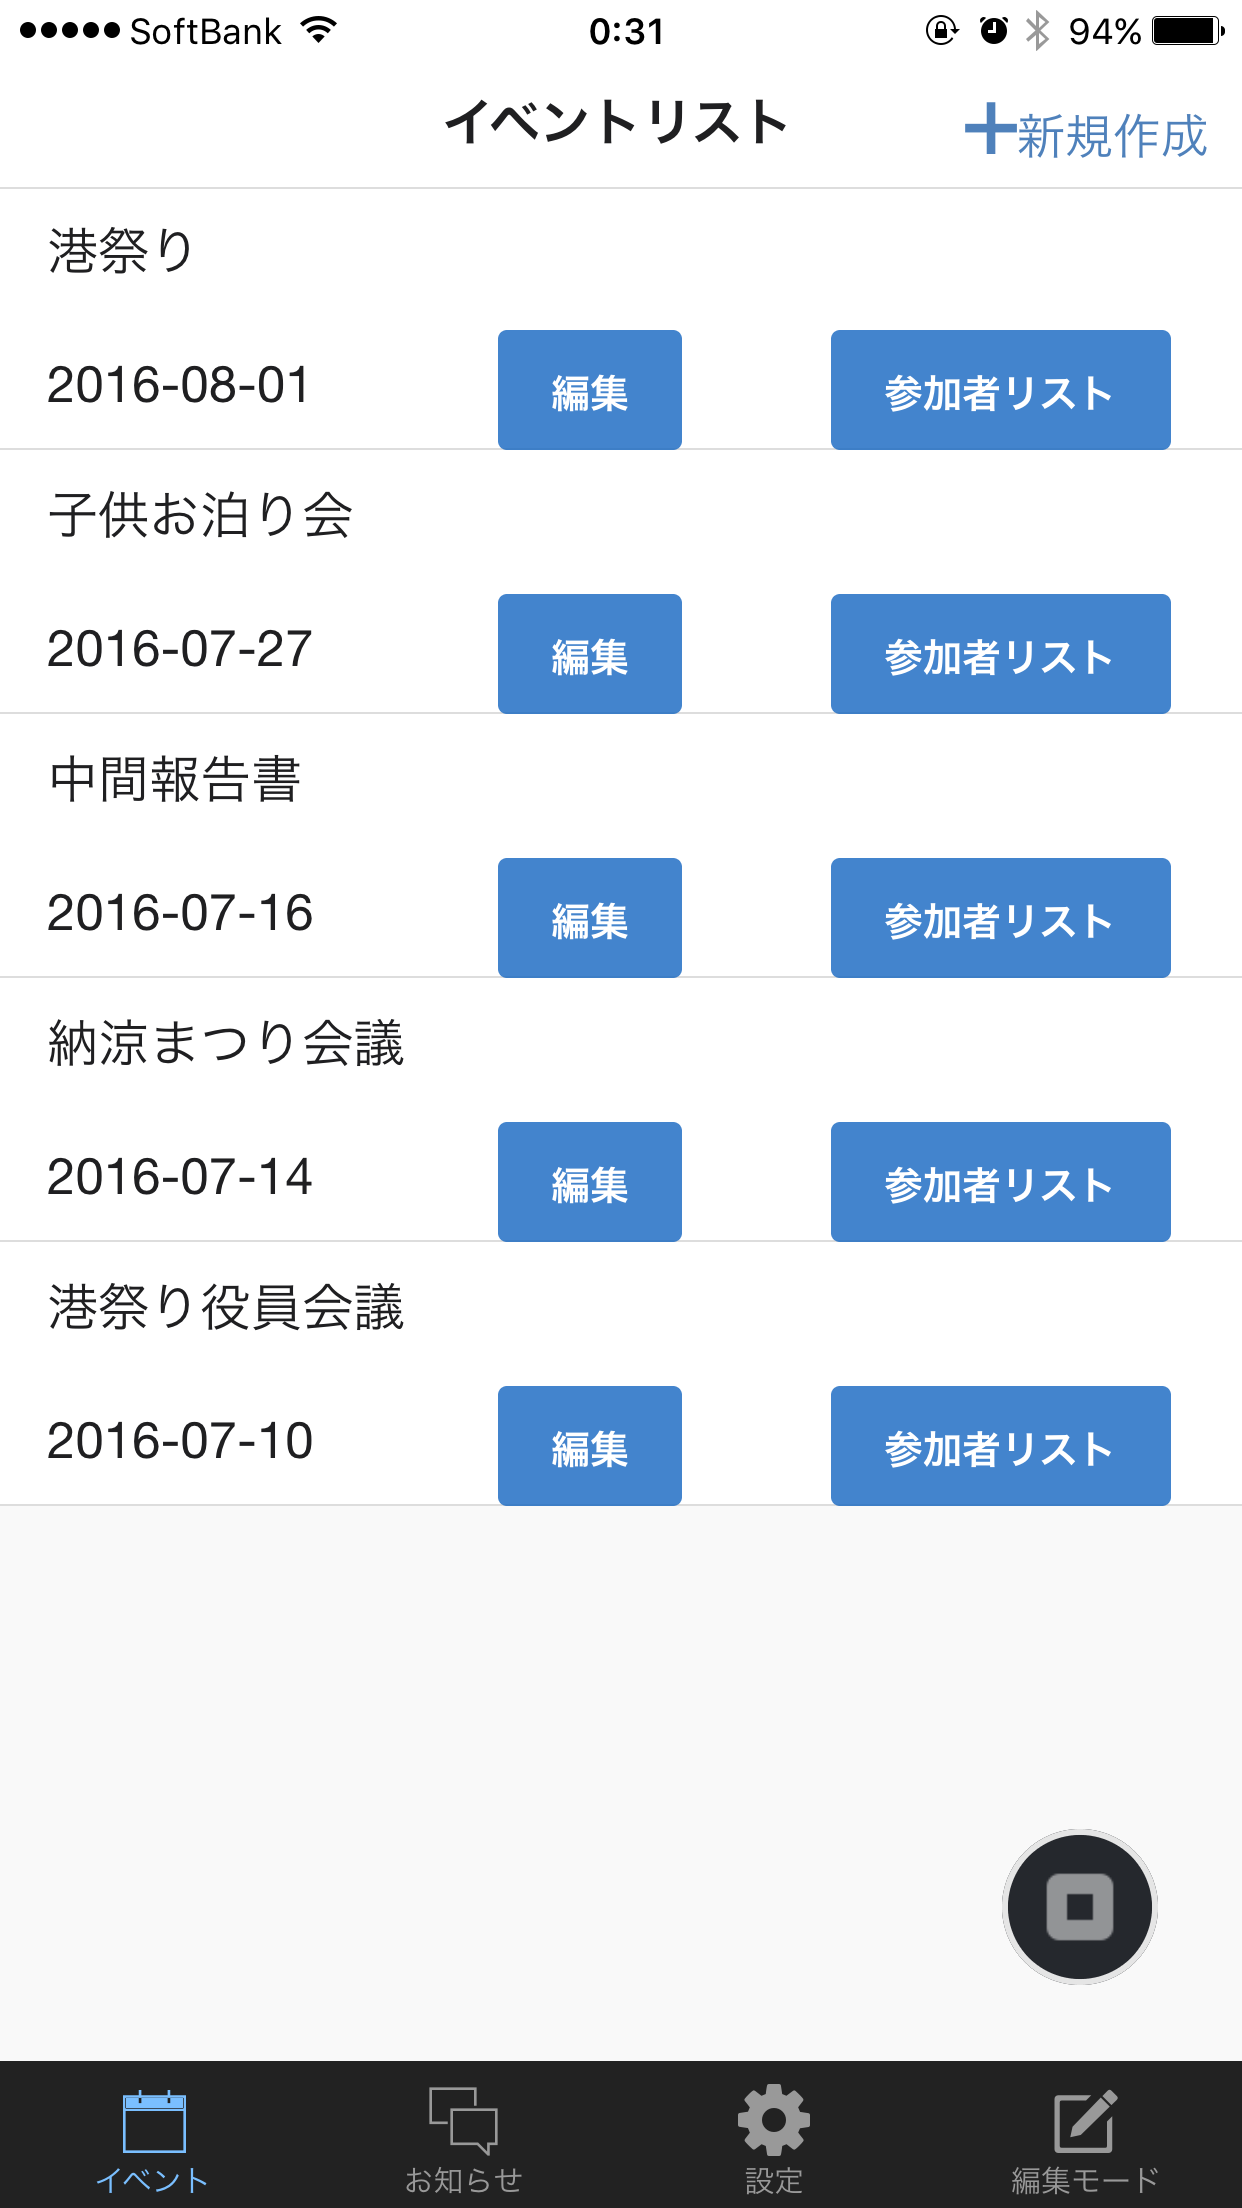
\includegraphics[width=4cm]{event_list.PNG}
          \hspace{1cm} %(a)観光スポットの紹介
          {\footnotesize (a)イベント一覧リスト画面}
        \end{center}
      \end{minipage}

      % 2
      \begin{minipage}{0.33\hsize}
        \begin{center}
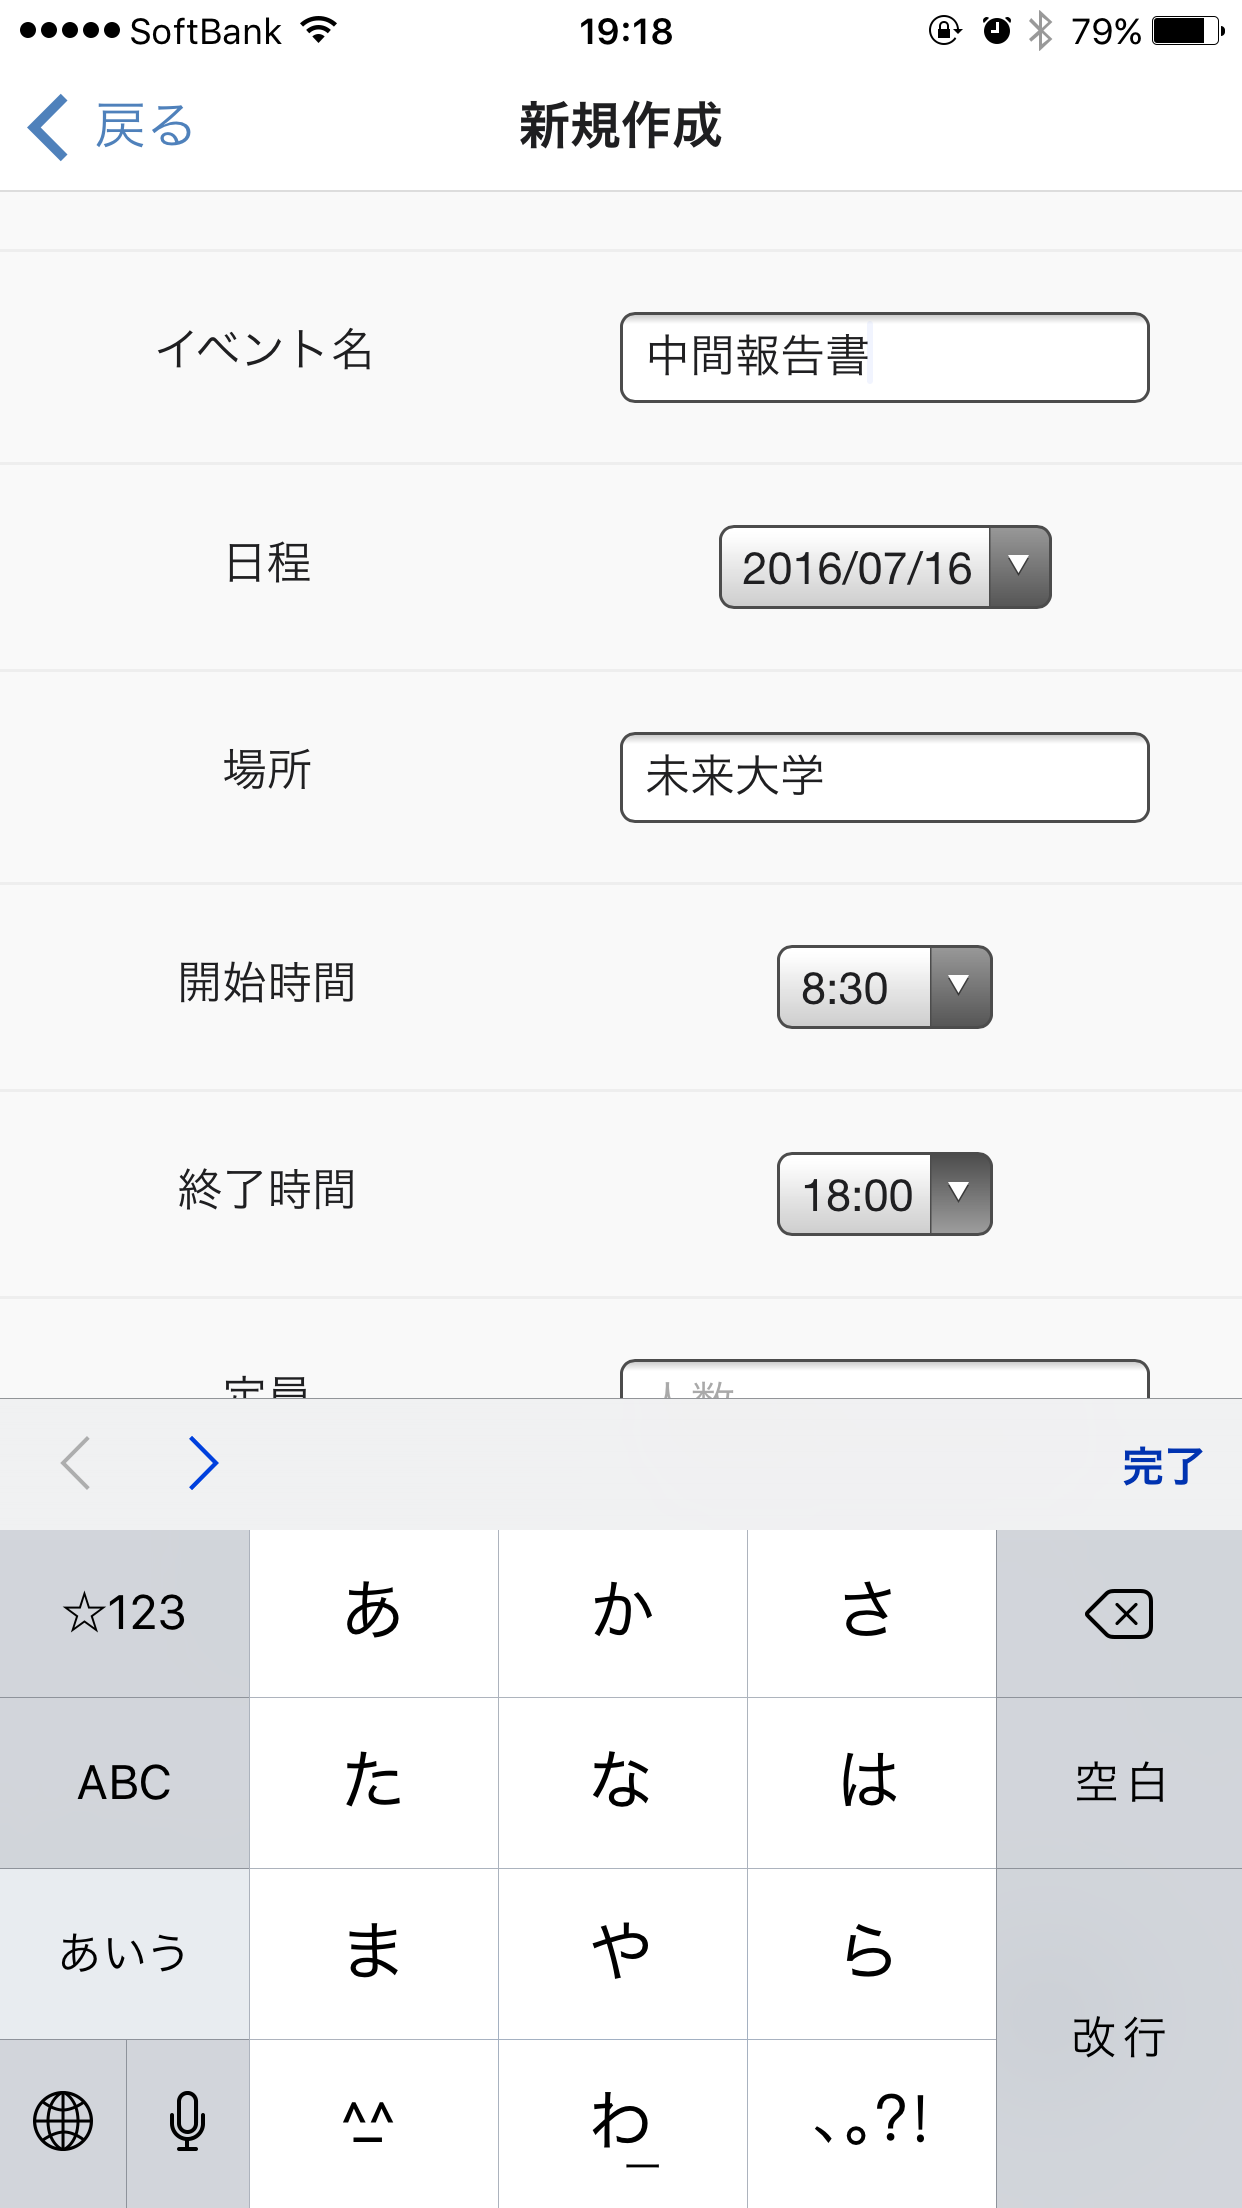
\includegraphics[width=4cm]{event_add.png}
          \hspace{1cm}% (b)観光スポットの詳細情報
          {\footnotesize (b)イベント情報の発信画面}
        \end{center}
      \end{minipage}

    \end{tabular}
    \caption{イベント情報の発信}
    \label{fig:lena}
  \end{center}
\end{figure}

\subsection{イベント情報の編集画面}%:発表技法について
イベント一覧リスト画面(図5.2(a))から任意の編集ボタンを押すと、イベント情報の編集画面(図5.2(b))に遷移する。イベント情報の編集画面では、イベント情報発信機能と同様に、8つの属性の情報を編集した後画面下の更新ボタンを押すことでイベント情報を再発信することが可能となる。また、画面下の削除ボタンを押すことでイベント情報の削除が可能となる。通知についてもイベント情報の発信機能と同様に行われる。

\begin{figure}[htbp]
  \begin{center}
    \begin{tabular}{c}

      % 1
      \begin{minipage}{0.33\hsize}
        \begin{center}
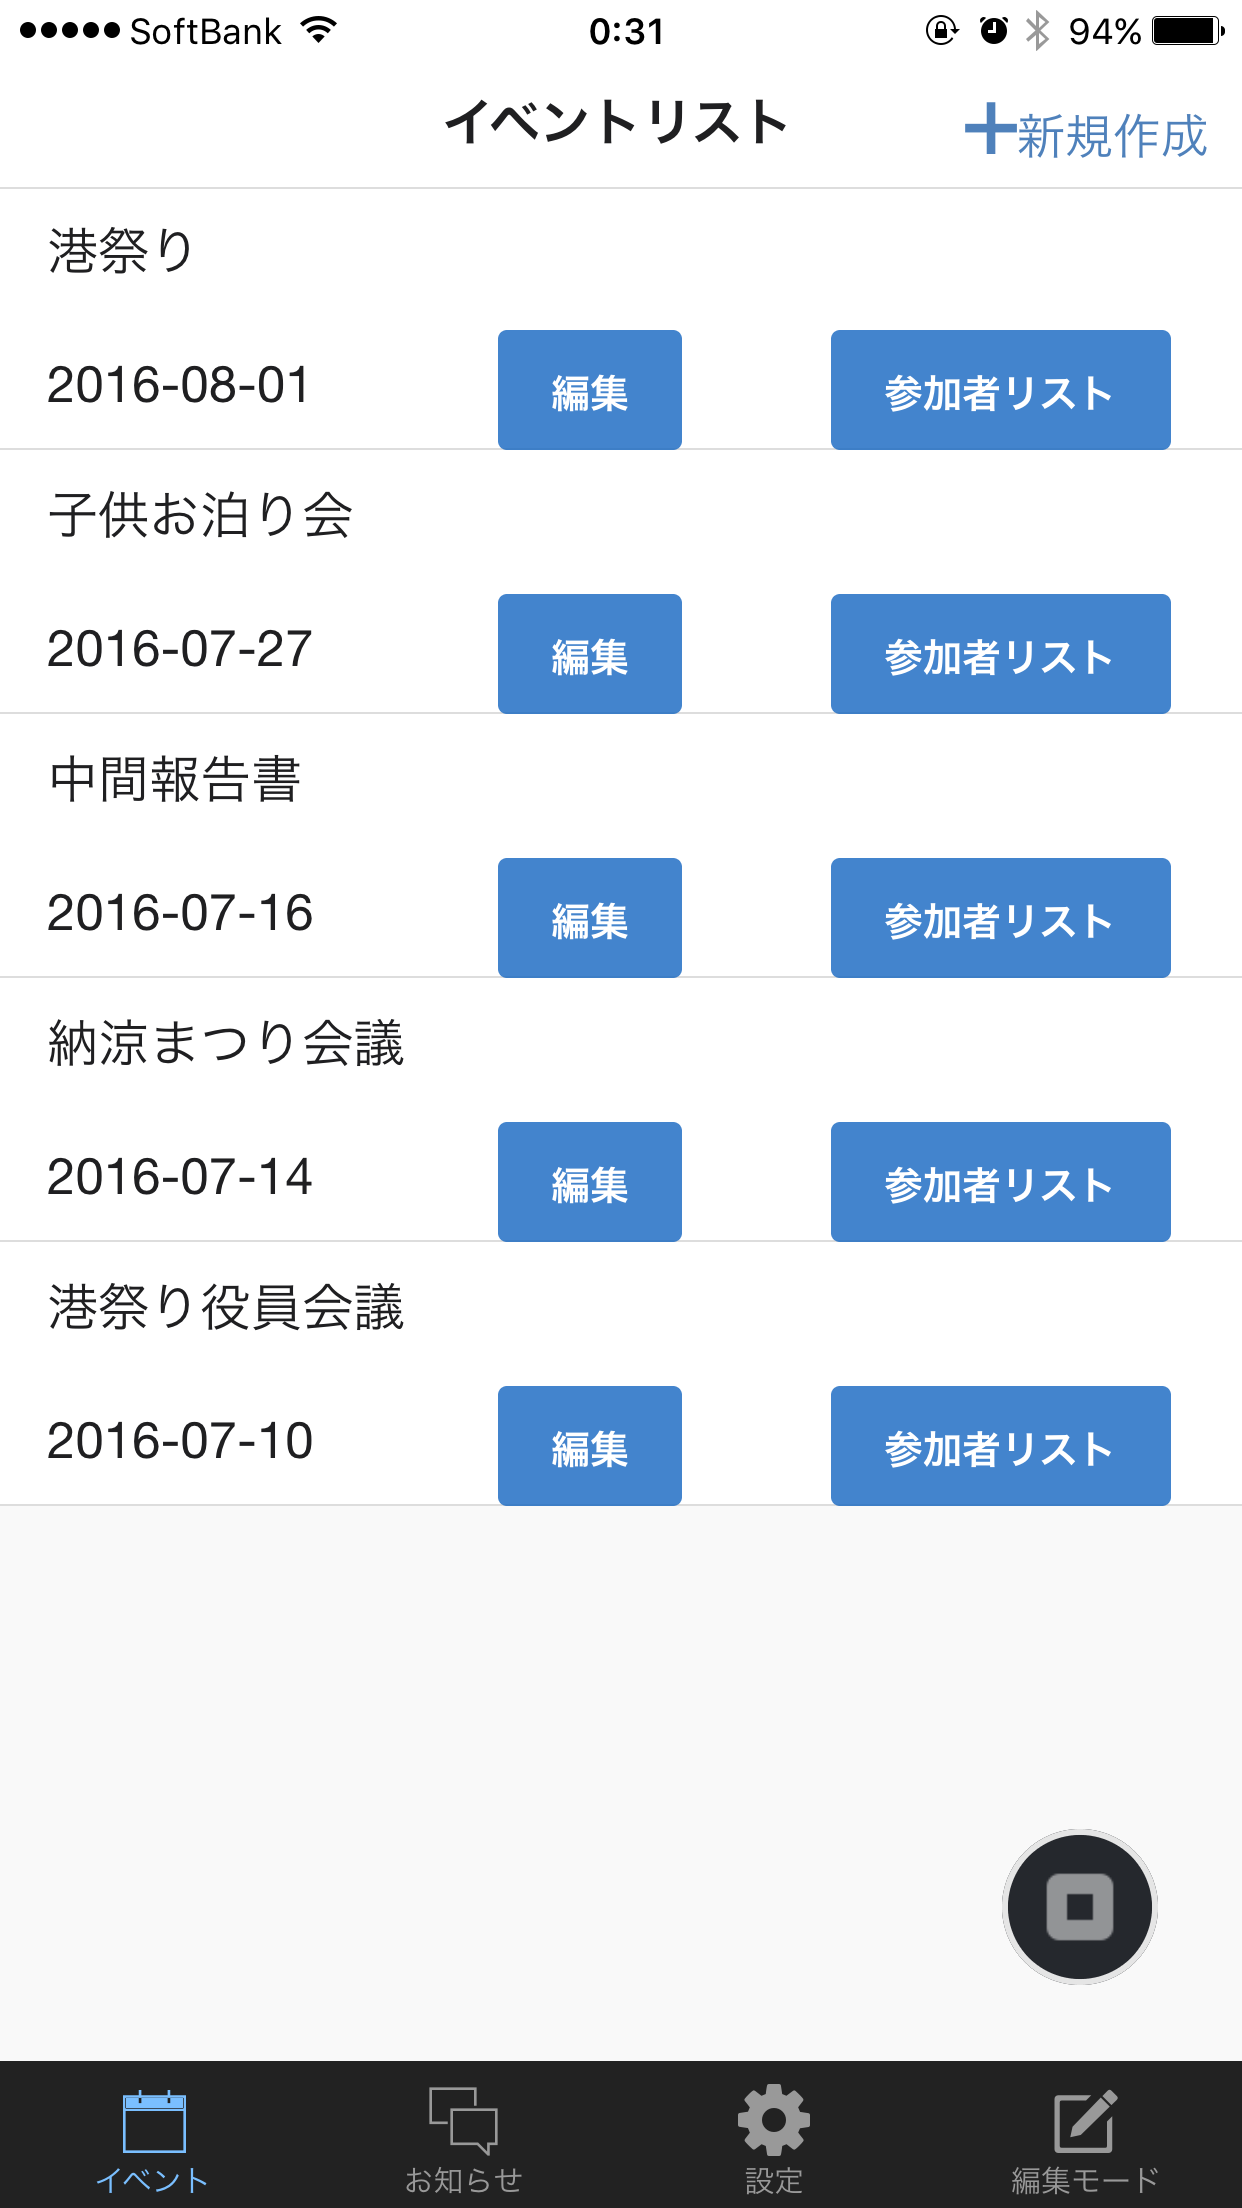
\includegraphics[width=4cm]{event_list.PNG}
          \hspace{1cm} %(a)観光スポットの紹介
          {\footnotesize (a)イベント一覧リスト画面}
        \end{center}
      \end{minipage}

      % 2
      \begin{minipage}{0.33\hsize}
        \begin{center}
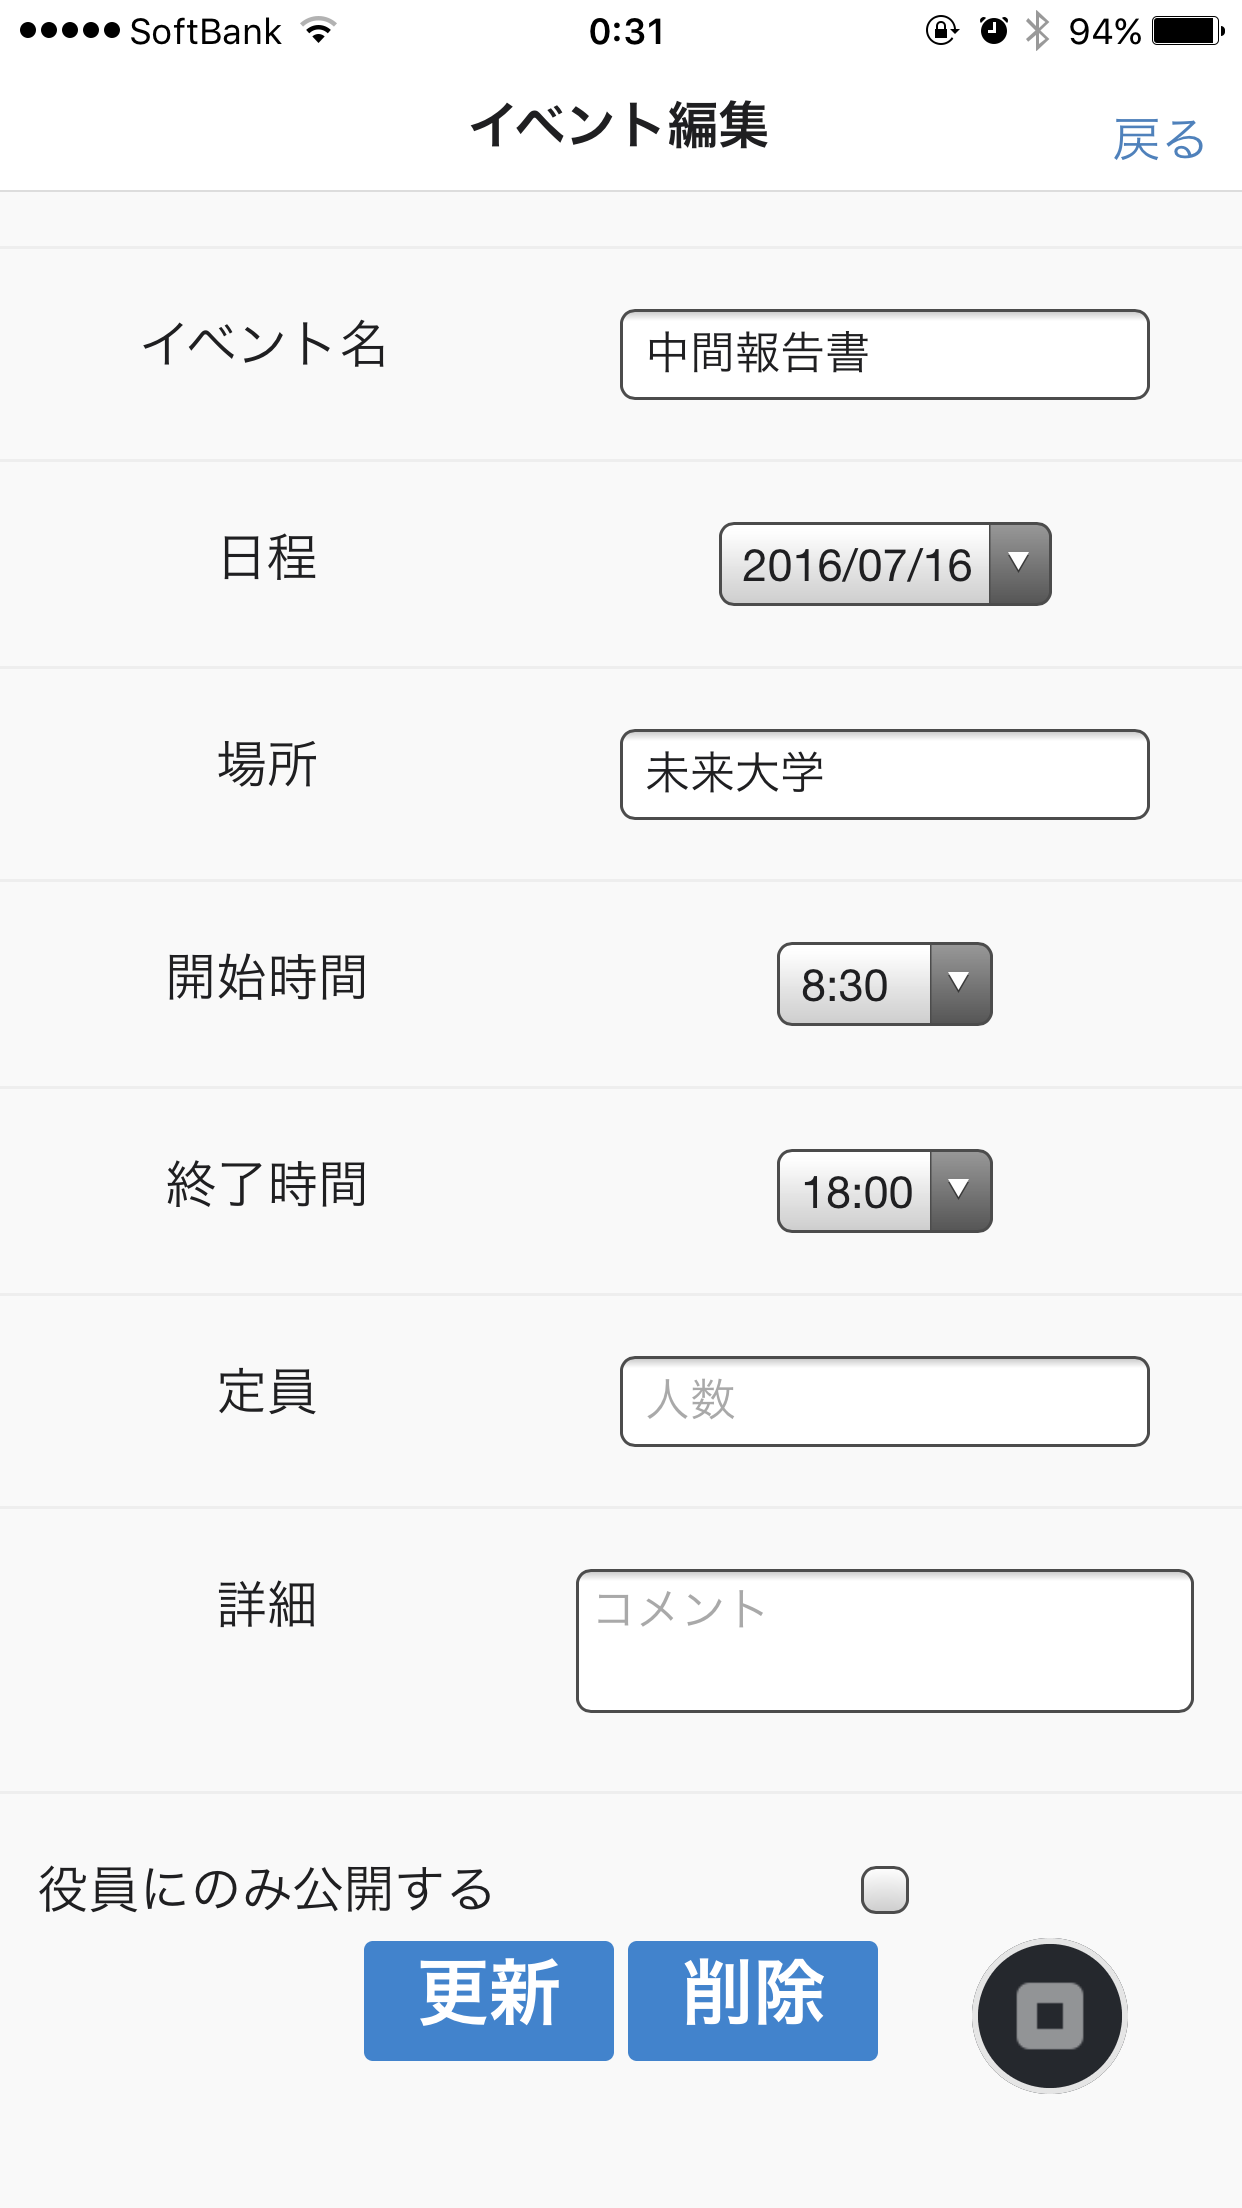
\includegraphics[width=4cm]{event_edit.PNG}
          \hspace{1cm}% (b)観光スポットの詳細情報
          {\footnotesize (b)イベント情報の編集画面}
        \end{center}
      \end{minipage}

    \end{tabular}
    \caption{イベント情報の編集}
    \label{fig:lena}
  \end{center}
\end{figure}

\section{イベント参加申し込み機能}%例:レビュー内容
\subsection{イベント参加申し込み機能の概要}%:発表技法について
イベント参加申し込み機能とは「一般モード」と「役員モード」の両方で可能な機能であり、主に発信されたイベントへの参加申し込みを行うことを可能とした。従来は、町民がイベントへの参加申し込みをする際に、電話、メール、FAX等多くの方法が存在していため、クライアントは参加者の管理に時間を要していた。イベント参加申し込み機能を実装した意図としては、この問題を解決し、クライアントの負荷を軽減するためである。

\subsection{イベント参加申し込み画面}%:発表技法について
イベント一覧リスト画面(図5.3(a))から参加ボタンを押すと、イベント参加申し込み画面(図5.3(b))に遷移する。イベント参加申し込み画面では、入力する情報の属性として氏名、性別、年齢、電話番号、住所の5つに分けた。これら5つの属性は、ヒアリングを通して定まったものである。情報を入力した後画面下の確定ボタンを押すことで参加申し込みが可能となる。また、家族など続けて参加申し込みをするケースを想定して、続けて参加申し込みを可能にした。その際、電話番号と住所欄には直前の情報を用いて入力済みとした。後期では続けて申し込みでなく、1度に連名での申し込みを可能にする予定である。

\begin{figure}[htbp]
  \begin{center}
    \begin{tabular}{c}

      % 1
      \begin{minipage}{0.33\hsize}
        \begin{center}
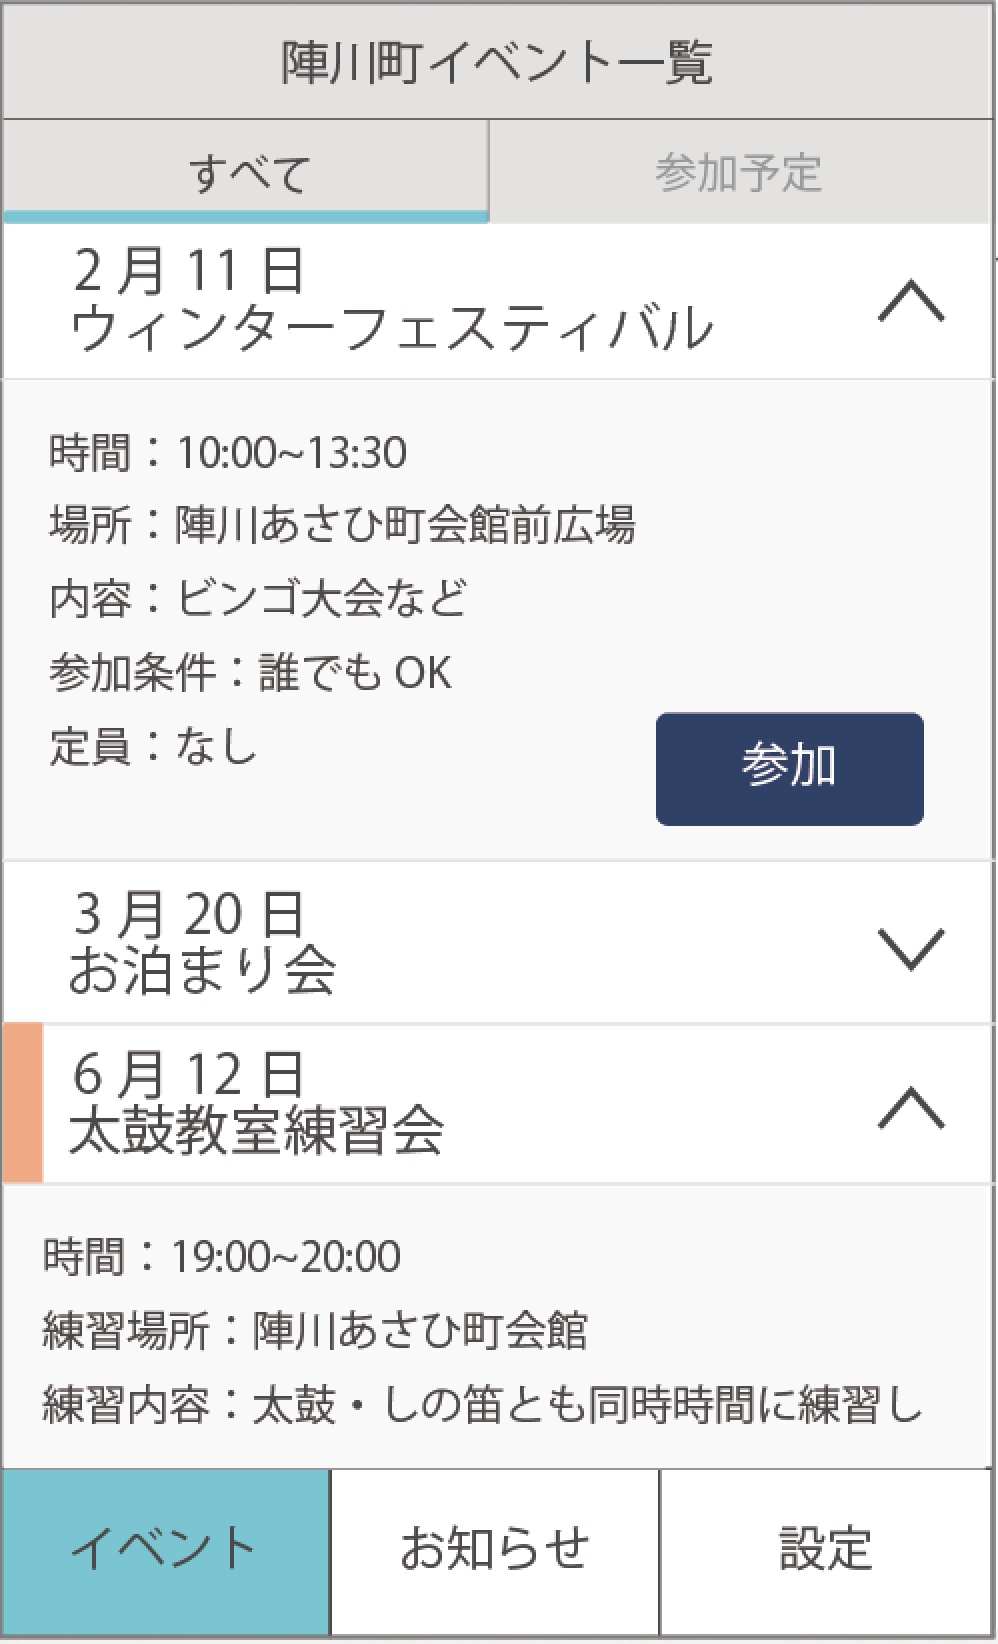
\includegraphics[width=4cm]{event_list_town.png}
          \hspace{1cm} %(a)観光スポットの紹介
          {\footnotesize (a)イベント一覧リスト画面}
        \end{center}
      \end{minipage}

      % 2
      \begin{minipage}{0.33\hsize}
        \begin{center}
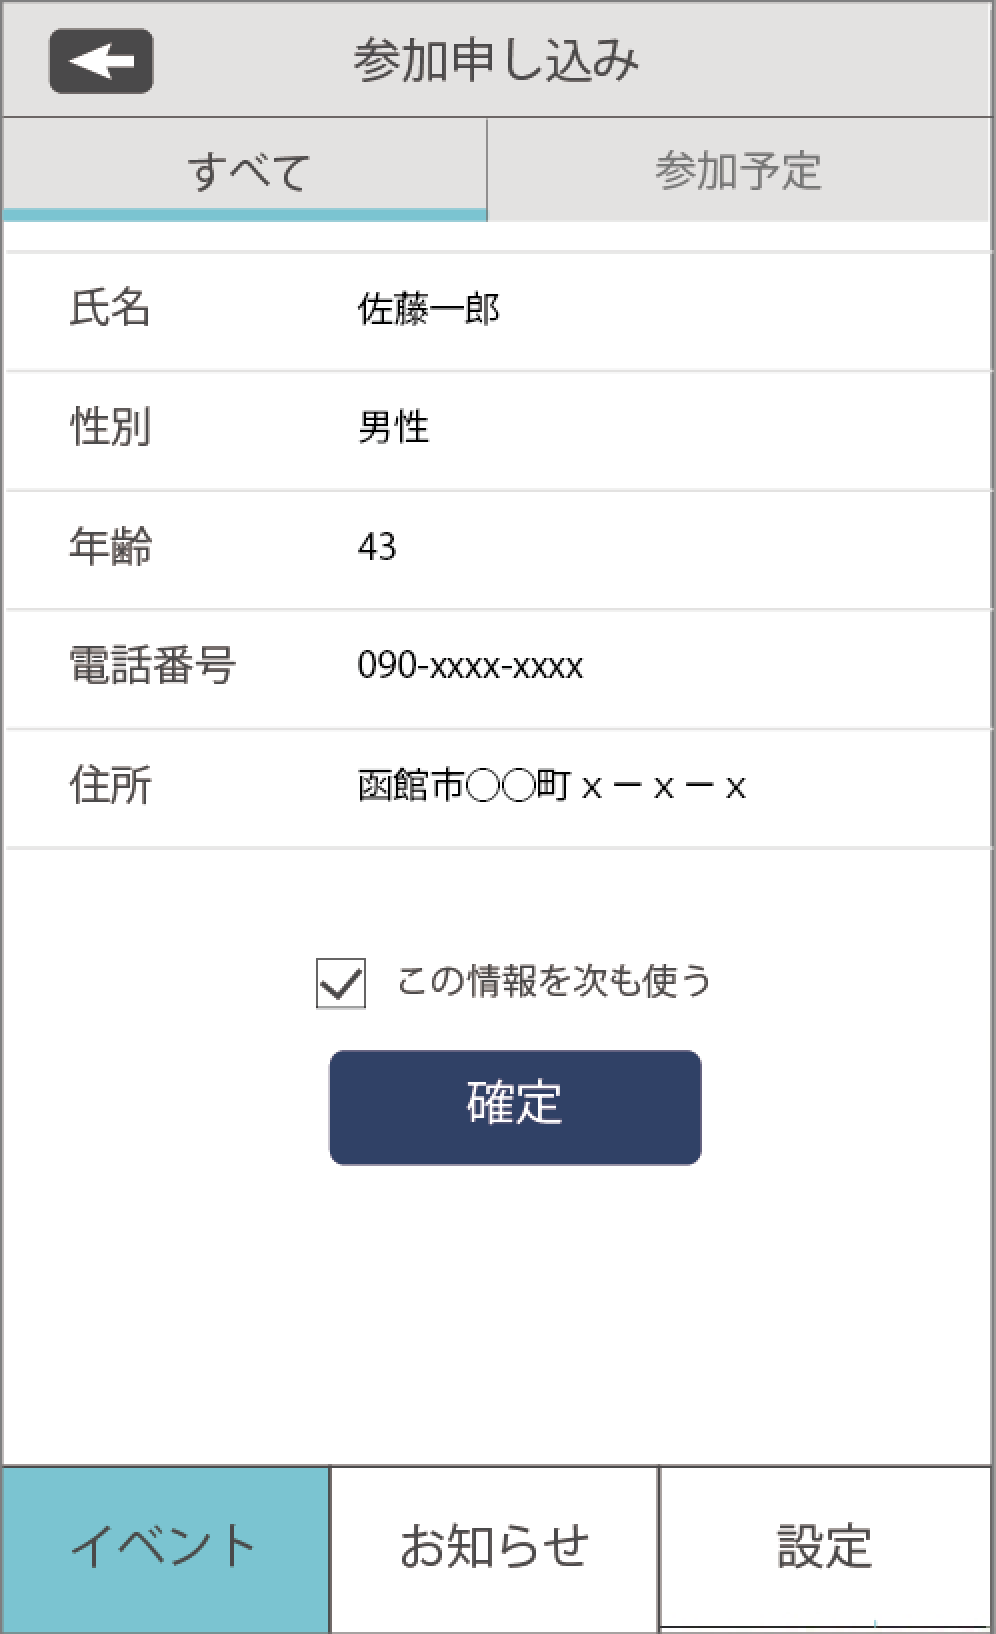
\includegraphics[width=4cm]{participant_form}
          \hspace{1cm}% (b)観光スポットの詳細情報
          {\footnotesize (b)イベント参加申し込み画面}
        \end{center}
      \end{minipage}

    \end{tabular}
    \caption{イベント参加申し込み}
    \label{fig:lena}
  \end{center}
\end{figure}

\section{参加者リスト画面}%例:レビュー内容
参加者リスト画面は「役員モード」でのみ閲覧可能な画面(図5.4(a))であり、イベント毎の参加者一覧の表示や参加取り消しを可能としている。また、画面上の追加参加ボタンを押すと、追加参加画面(図5.4(b))に遷移する。実装した意図としては、イベント参加申し込み機能と同様にクライアントの負荷を軽減するためである。追加参加画面では、役員が本アプリケーションを使用することができないユーザの代わりに参加申し込みをすることを可能にした。また、クライアントへのヒアリングの結果、参加者リストを市役所に提出する必要があるイベントが存在することがわかった。これを楽に行えるように、後期では参加者リストのCSVファイル形式での出力機能を実装する予定である。

\begin{figure}[htbp]
  \begin{center}
    \begin{tabular}{c}

      % 1
      \begin{minipage}{0.33\hsize}
        \begin{center}
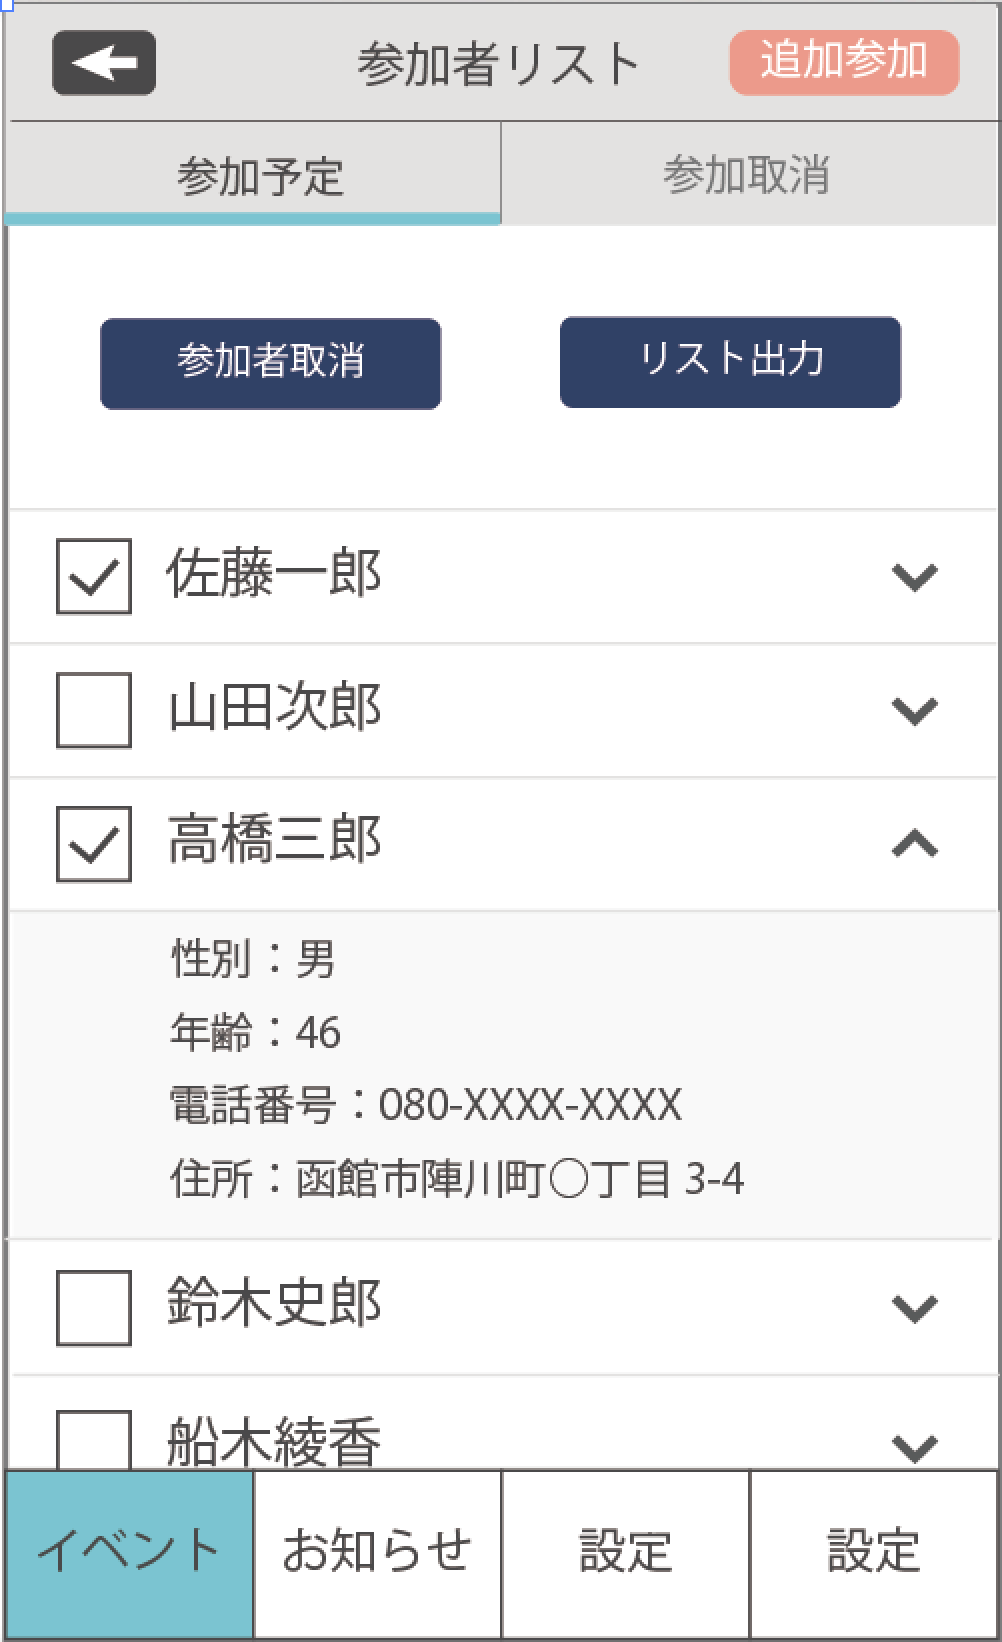
\includegraphics[width=4cm]{participant_list}
          \hspace{1cm} %(a)観光スポットの紹介
          {\footnotesize (a)参加者リスト画面}
        \end{center}
      \end{minipage}

      % 2
      \begin{minipage}{0.33\hsize}
        \begin{center}
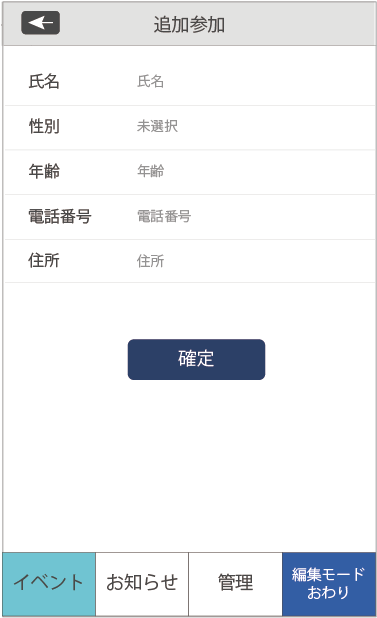
\includegraphics[width=4cm]{participant_add.png}
          \hspace{1cm}% (b)観光スポットの詳細情報
          {\footnotesize (b)追加参加画面}
        \end{center}
      \end{minipage}

    \end{tabular}
    \caption{参加者リスト}
    \label{fig:lena}
  \end{center}
\end{figure}

\section{おしらせ管理機能}%例:レビュー内容
\subsection{おしらせ管理機能の概要}%:発表技法について
おしらせ管理機能とは「役員モード」での利用可能な機能であり、陣川あさひ町会からのお知らせを発信、発信したお知らせの削除を可能とした。これらは、役員のうち編集者のみが使うことを可能とした。編集者のみとした理由は、イベント管理機能と同様の理由である。おしらせ機能を実装した意図としては、1.2節でも記述したが過去のイベントで雨天中止の連絡が出来なかったために、参加者に風邪を引かせてしまったという事例が合ったことから、町会からのお知らせを迅速に参加者に伝える必要があると判断したからである。またこの機能を用いて、「今日は燃えるゴミが出せる日」「午後から雨が振るので、洗濯物は取り込んでおいて下さい」といった生活情報の発信も行うことが可能となる。


\subsection{お知らせ作成画面}%:発表技法について
お知らせ一覧リスト画面(図5.5(a))から新規作成ボタンを押すと、お知らせの新規作成画面(図5.5(b))に遷移する。お知らせの新規作成画面では、お知らせ内容を入力し役員のみに公開するか否かを選択した後画面下の作成ボタンを押すことでお知らせを発信することが可能となる。通知についても他と同様に行われる。

\begin{figure}[htbp]
  \begin{center}
    \begin{tabular}{c}

      % 1
      \begin{minipage}{0.33\hsize}
        \begin{center}
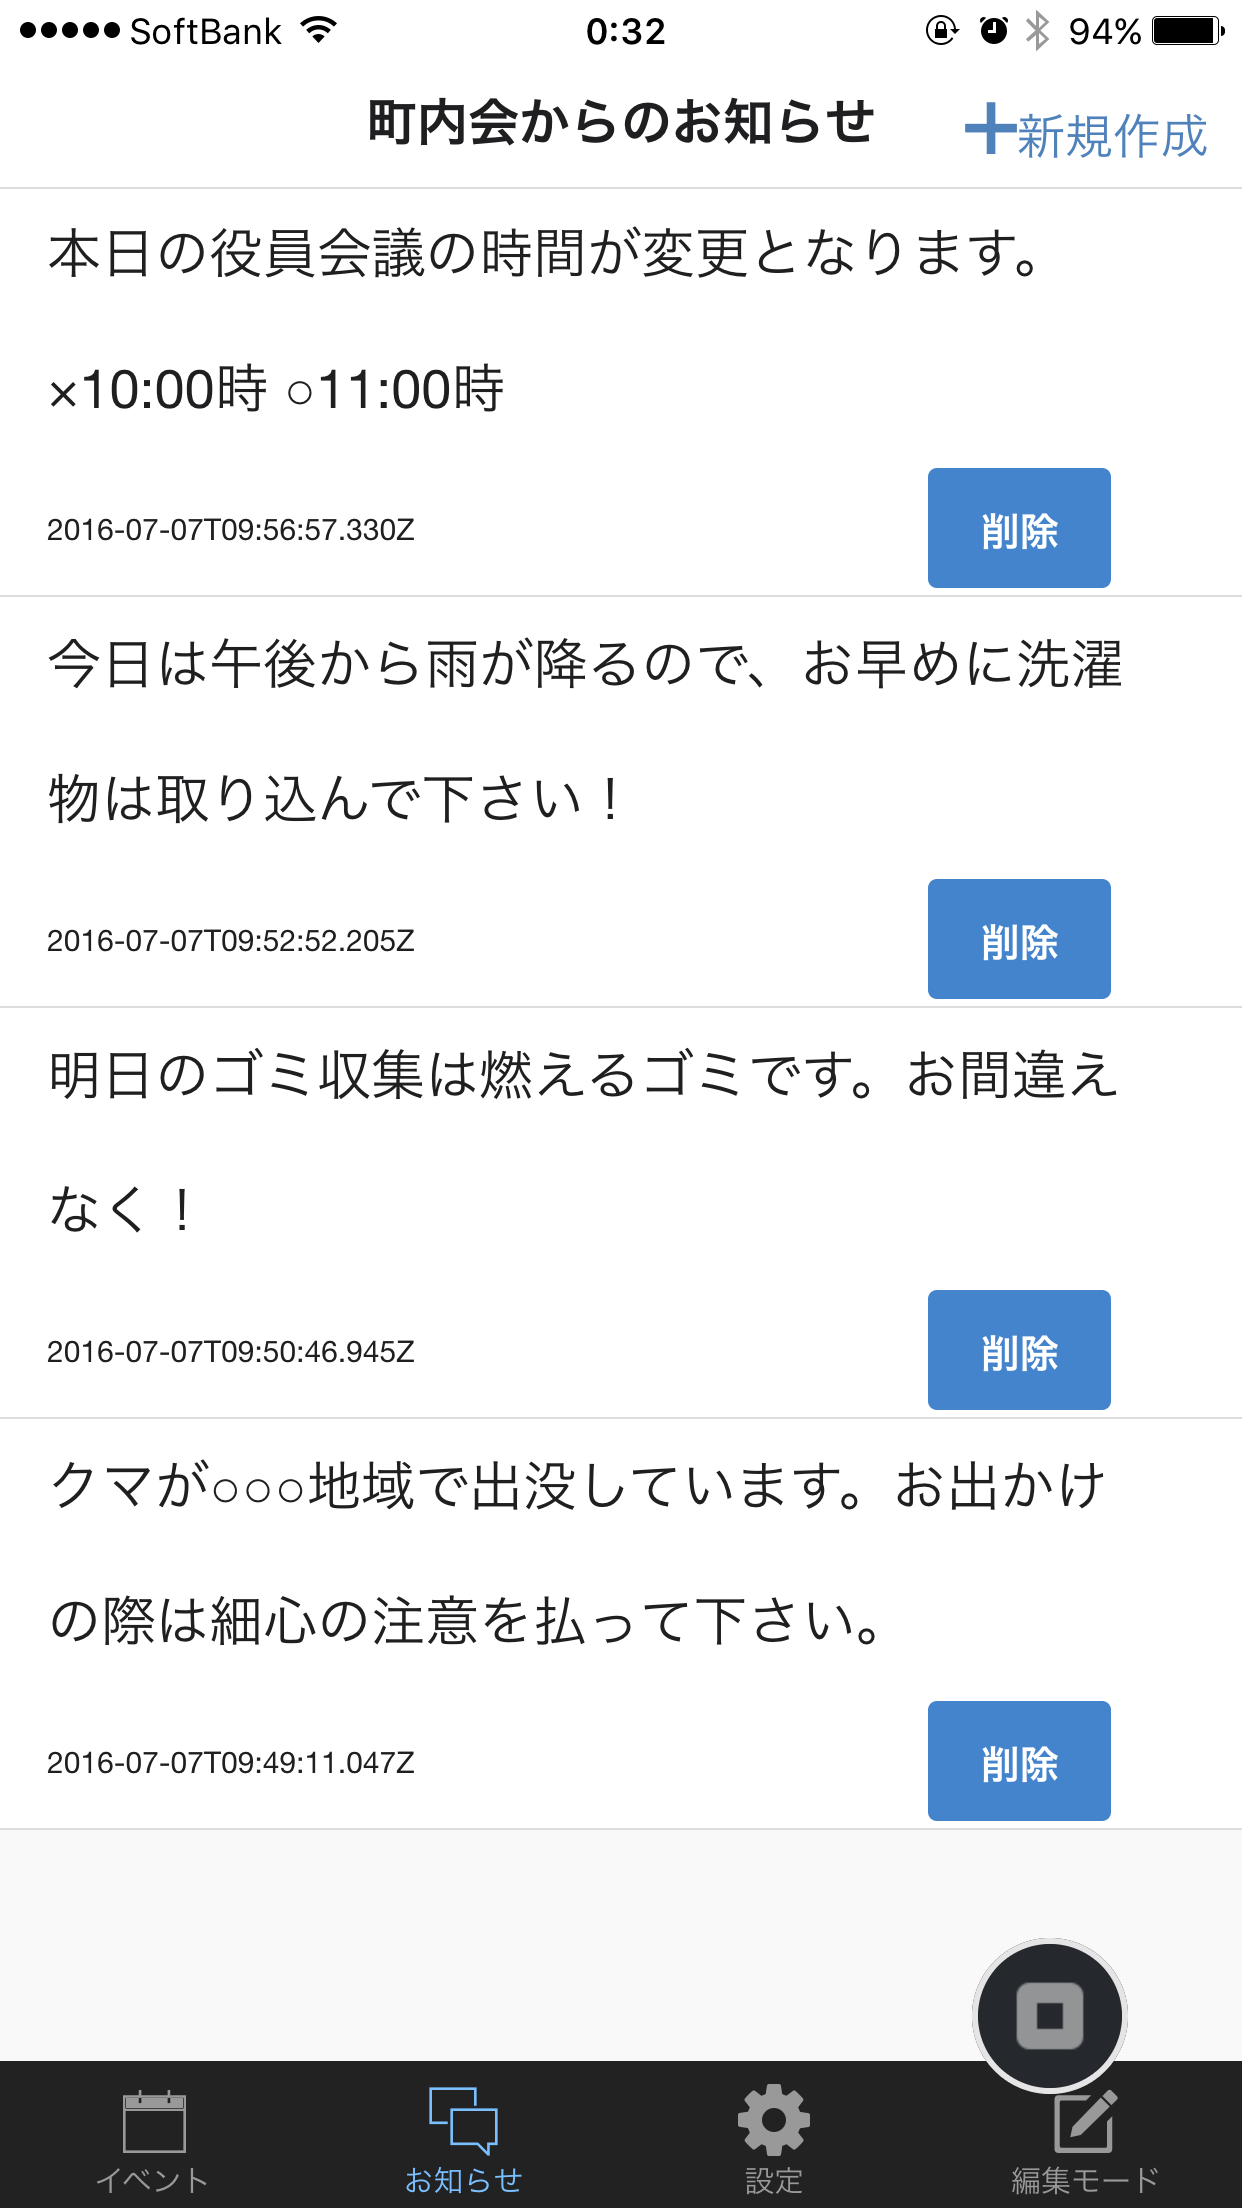
\includegraphics[width=4cm]{notification_list.PNG}
          \hspace{1cm} %(a)観光スポットの紹介
          {\footnotesize (a)お知らせ一覧リスト画面}
        \end{center}
      \end{minipage}

      % 2
      \begin{minipage}{0.33\hsize}
        \begin{center}
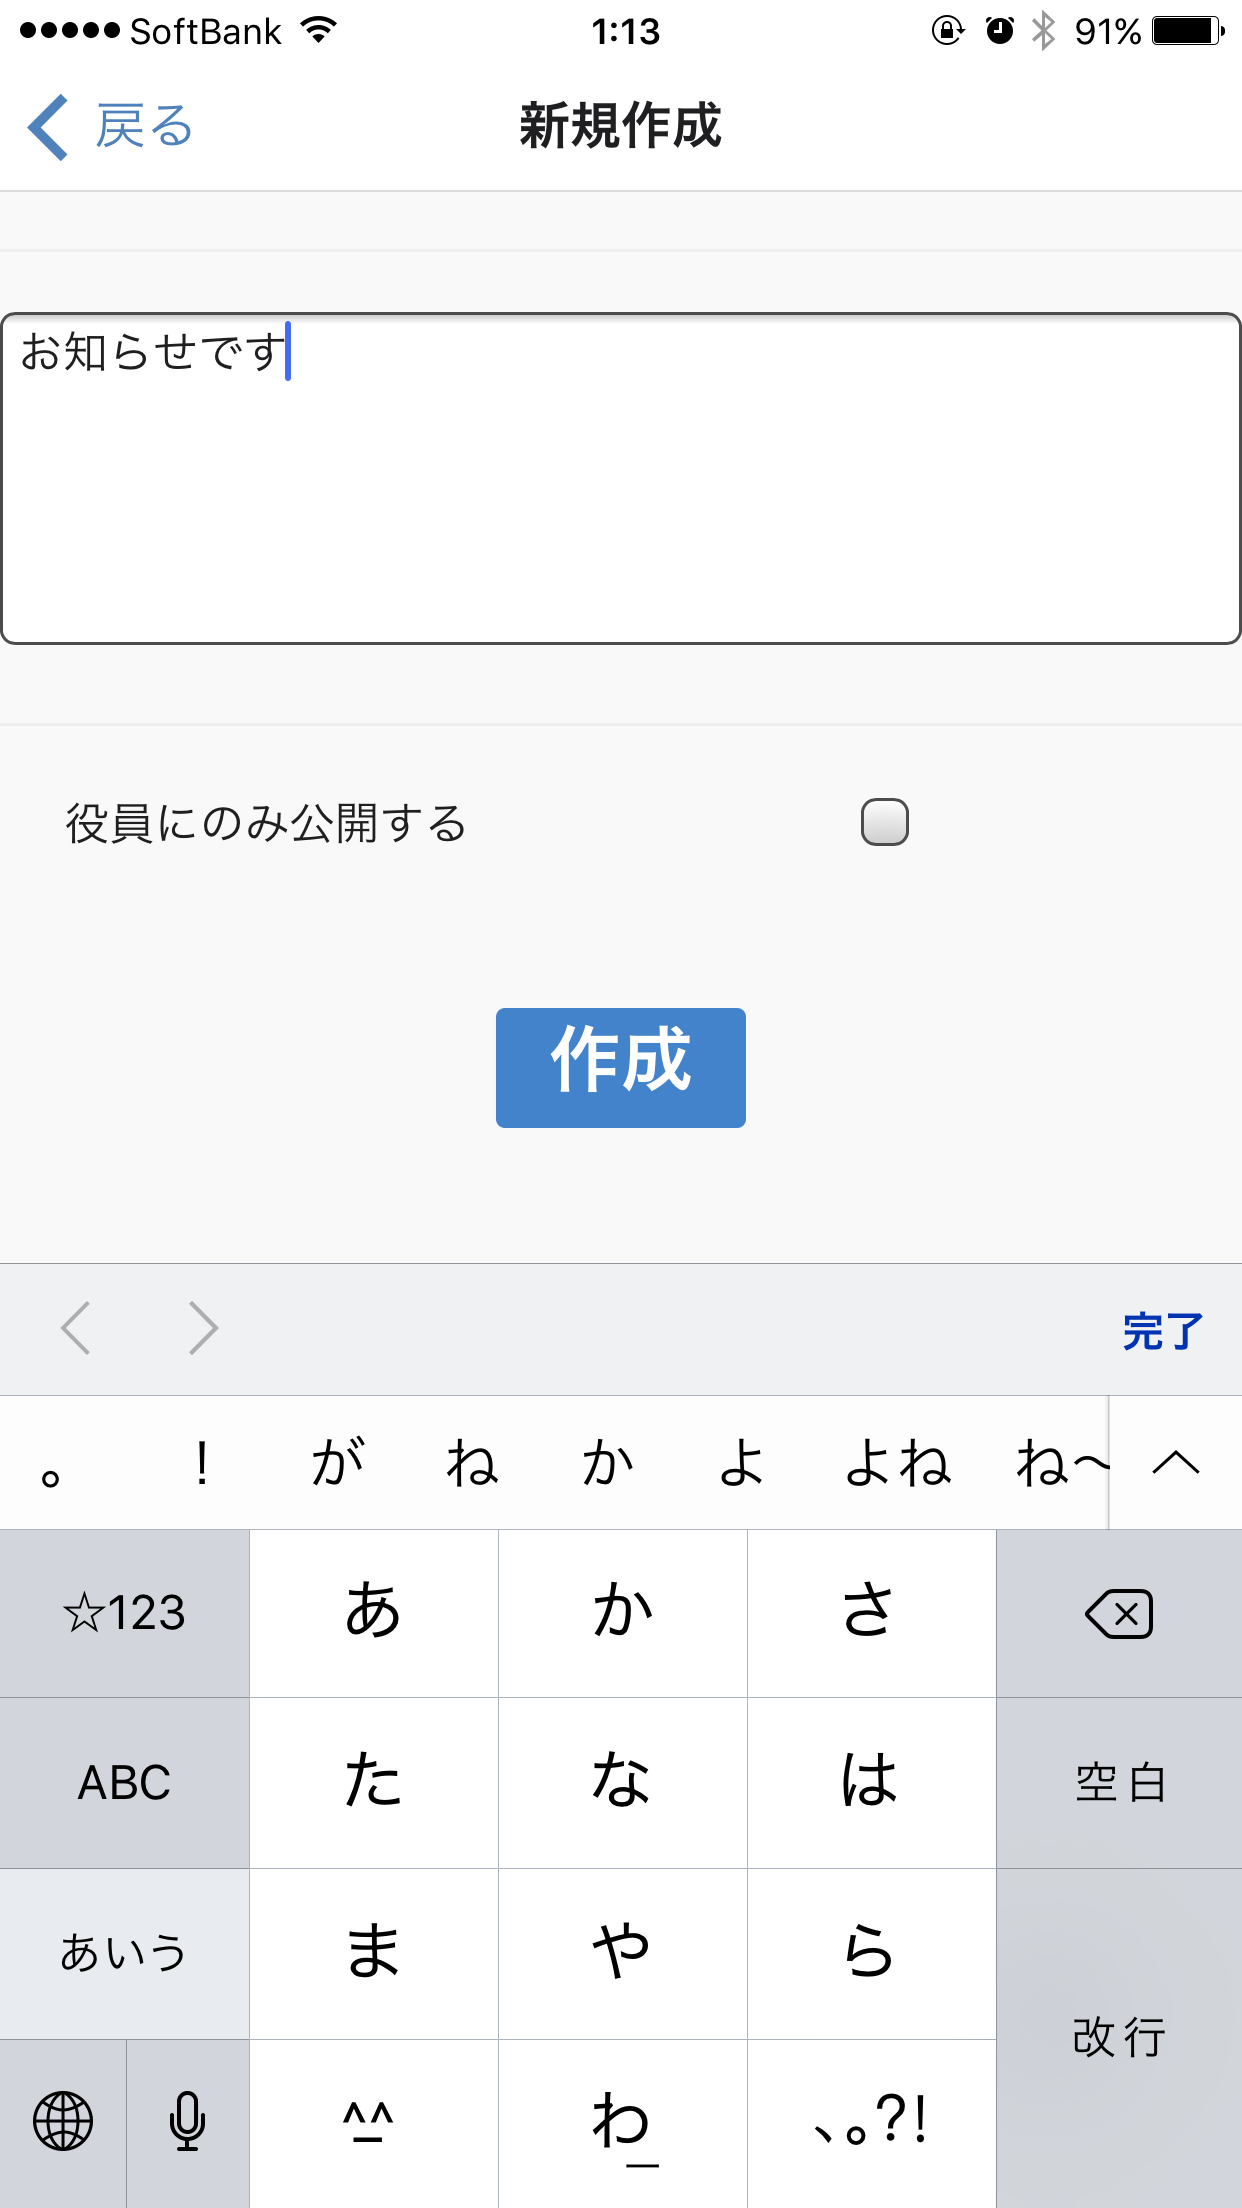
\includegraphics[width=4cm]{notification_add.PNG}
          \hspace{1cm}% (b)観光スポットの詳細情報
          {\footnotesize (b)お知らせの新規作成画面}
        \end{center}
      \end{minipage}

    \end{tabular}
    \caption{お知らせ作成}
    \label{fig:lena}
  \end{center}
\end{figure}

\subsection{お知らせ削除}%:発表技法について
お知らせ一覧リスト画面(図5.6(a))から削除ボタンを選択して、発信した任意のお知らせの削除を行う(図5.6(b))。

\begin{figure}[htbp]
  \begin{center}
    \begin{tabular}{c}

      % 1
      \begin{minipage}{0.33\hsize}
        \begin{center}
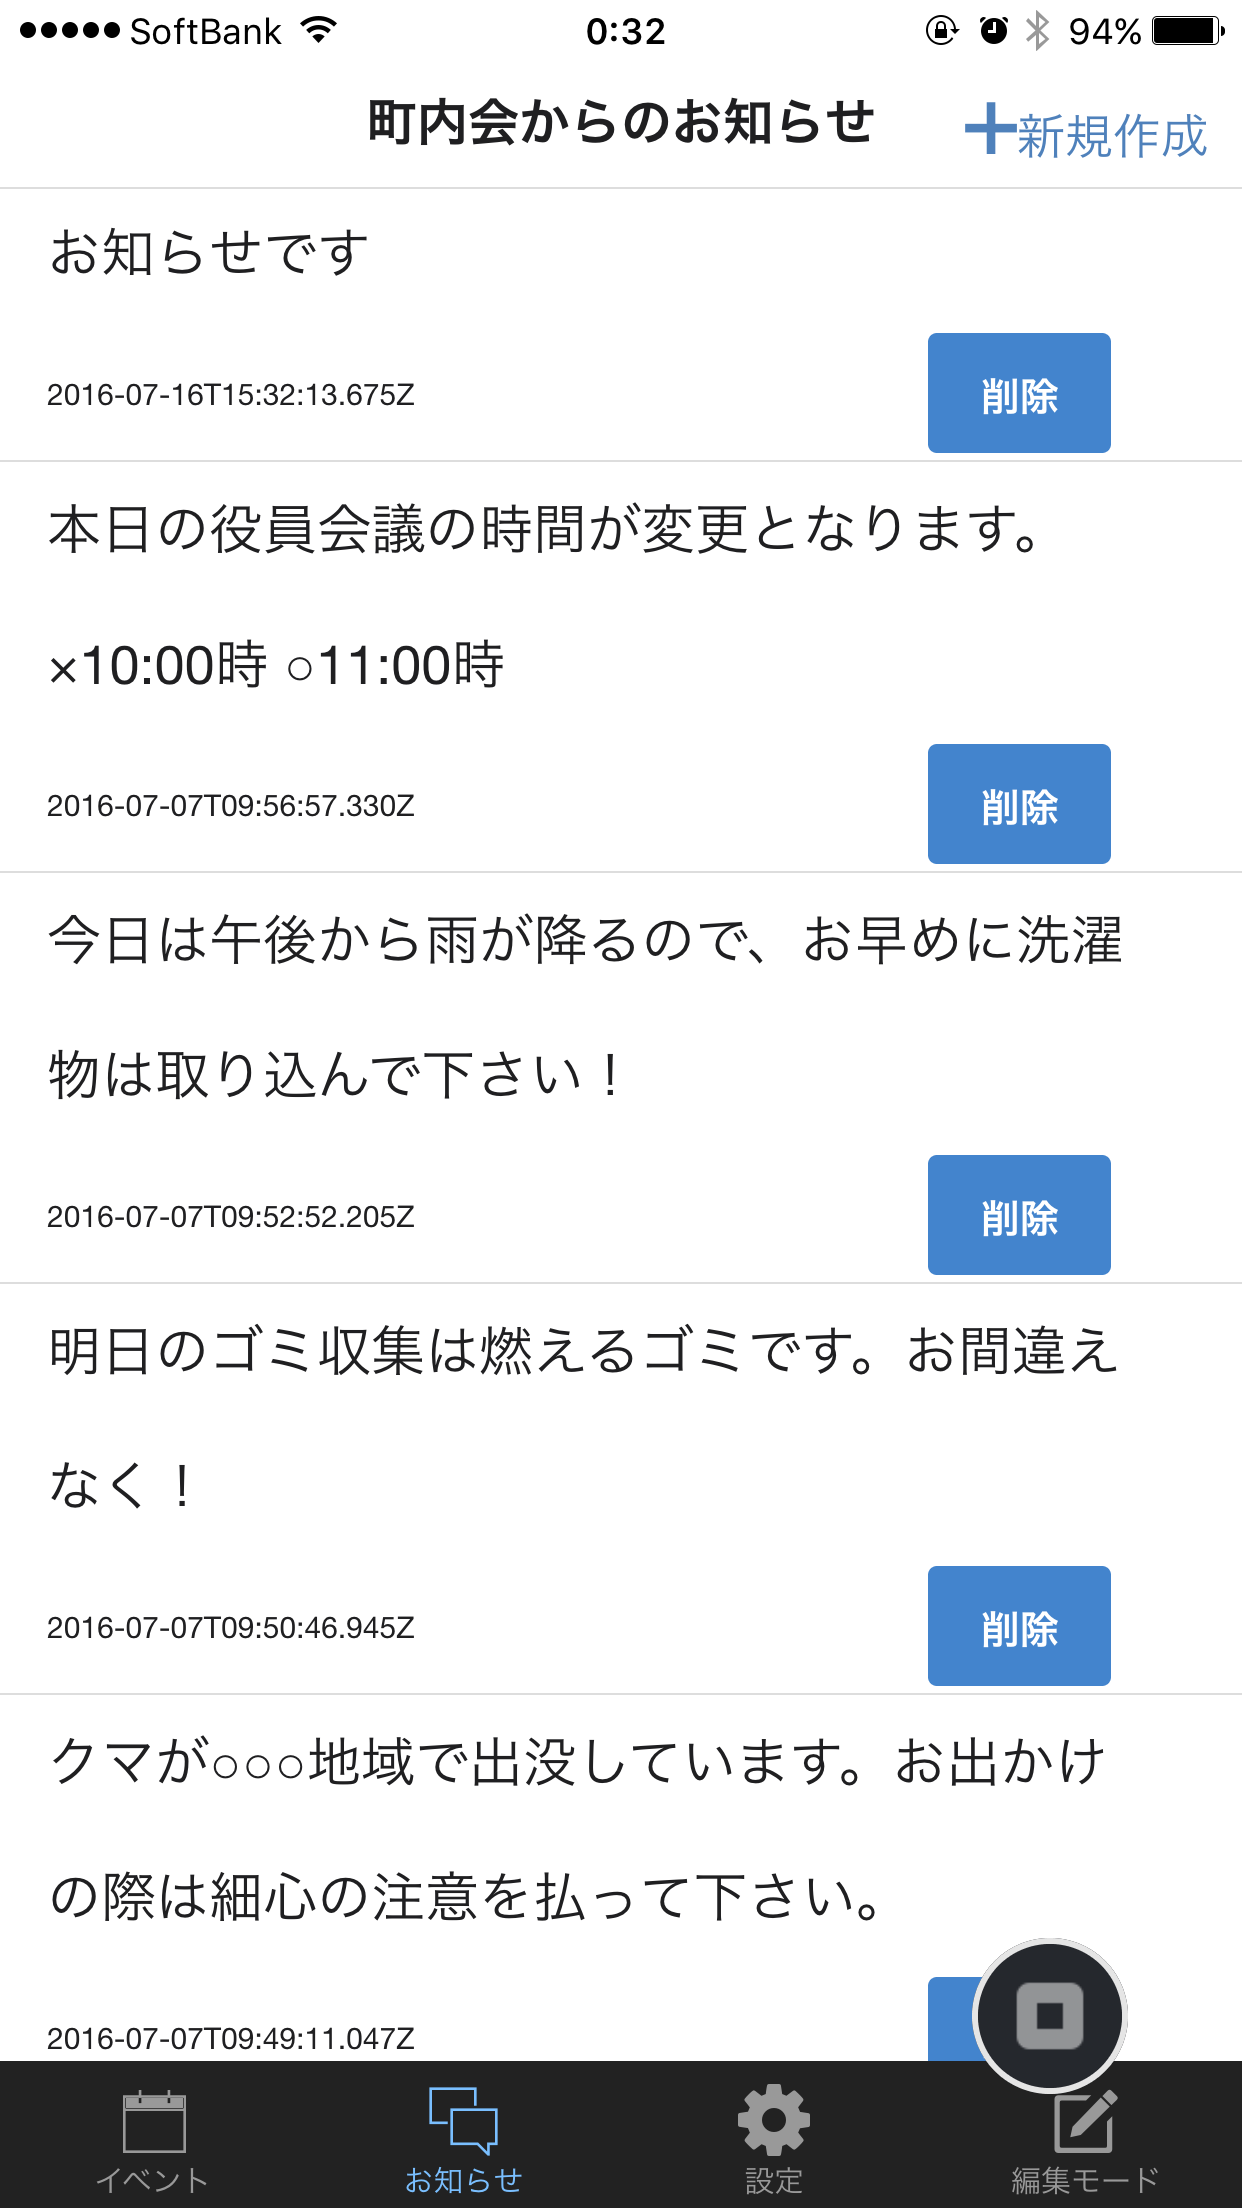
\includegraphics[width=4cm]{notification_list_after_add.PNG}
          \hspace{1cm} %(a)観光スポットの紹介
          {\footnotesize (a)お知らせ一覧リスト画面}
        \end{center}
      \end{minipage}

      % 2
      \begin{minipage}{0.33\hsize}
        \begin{center}
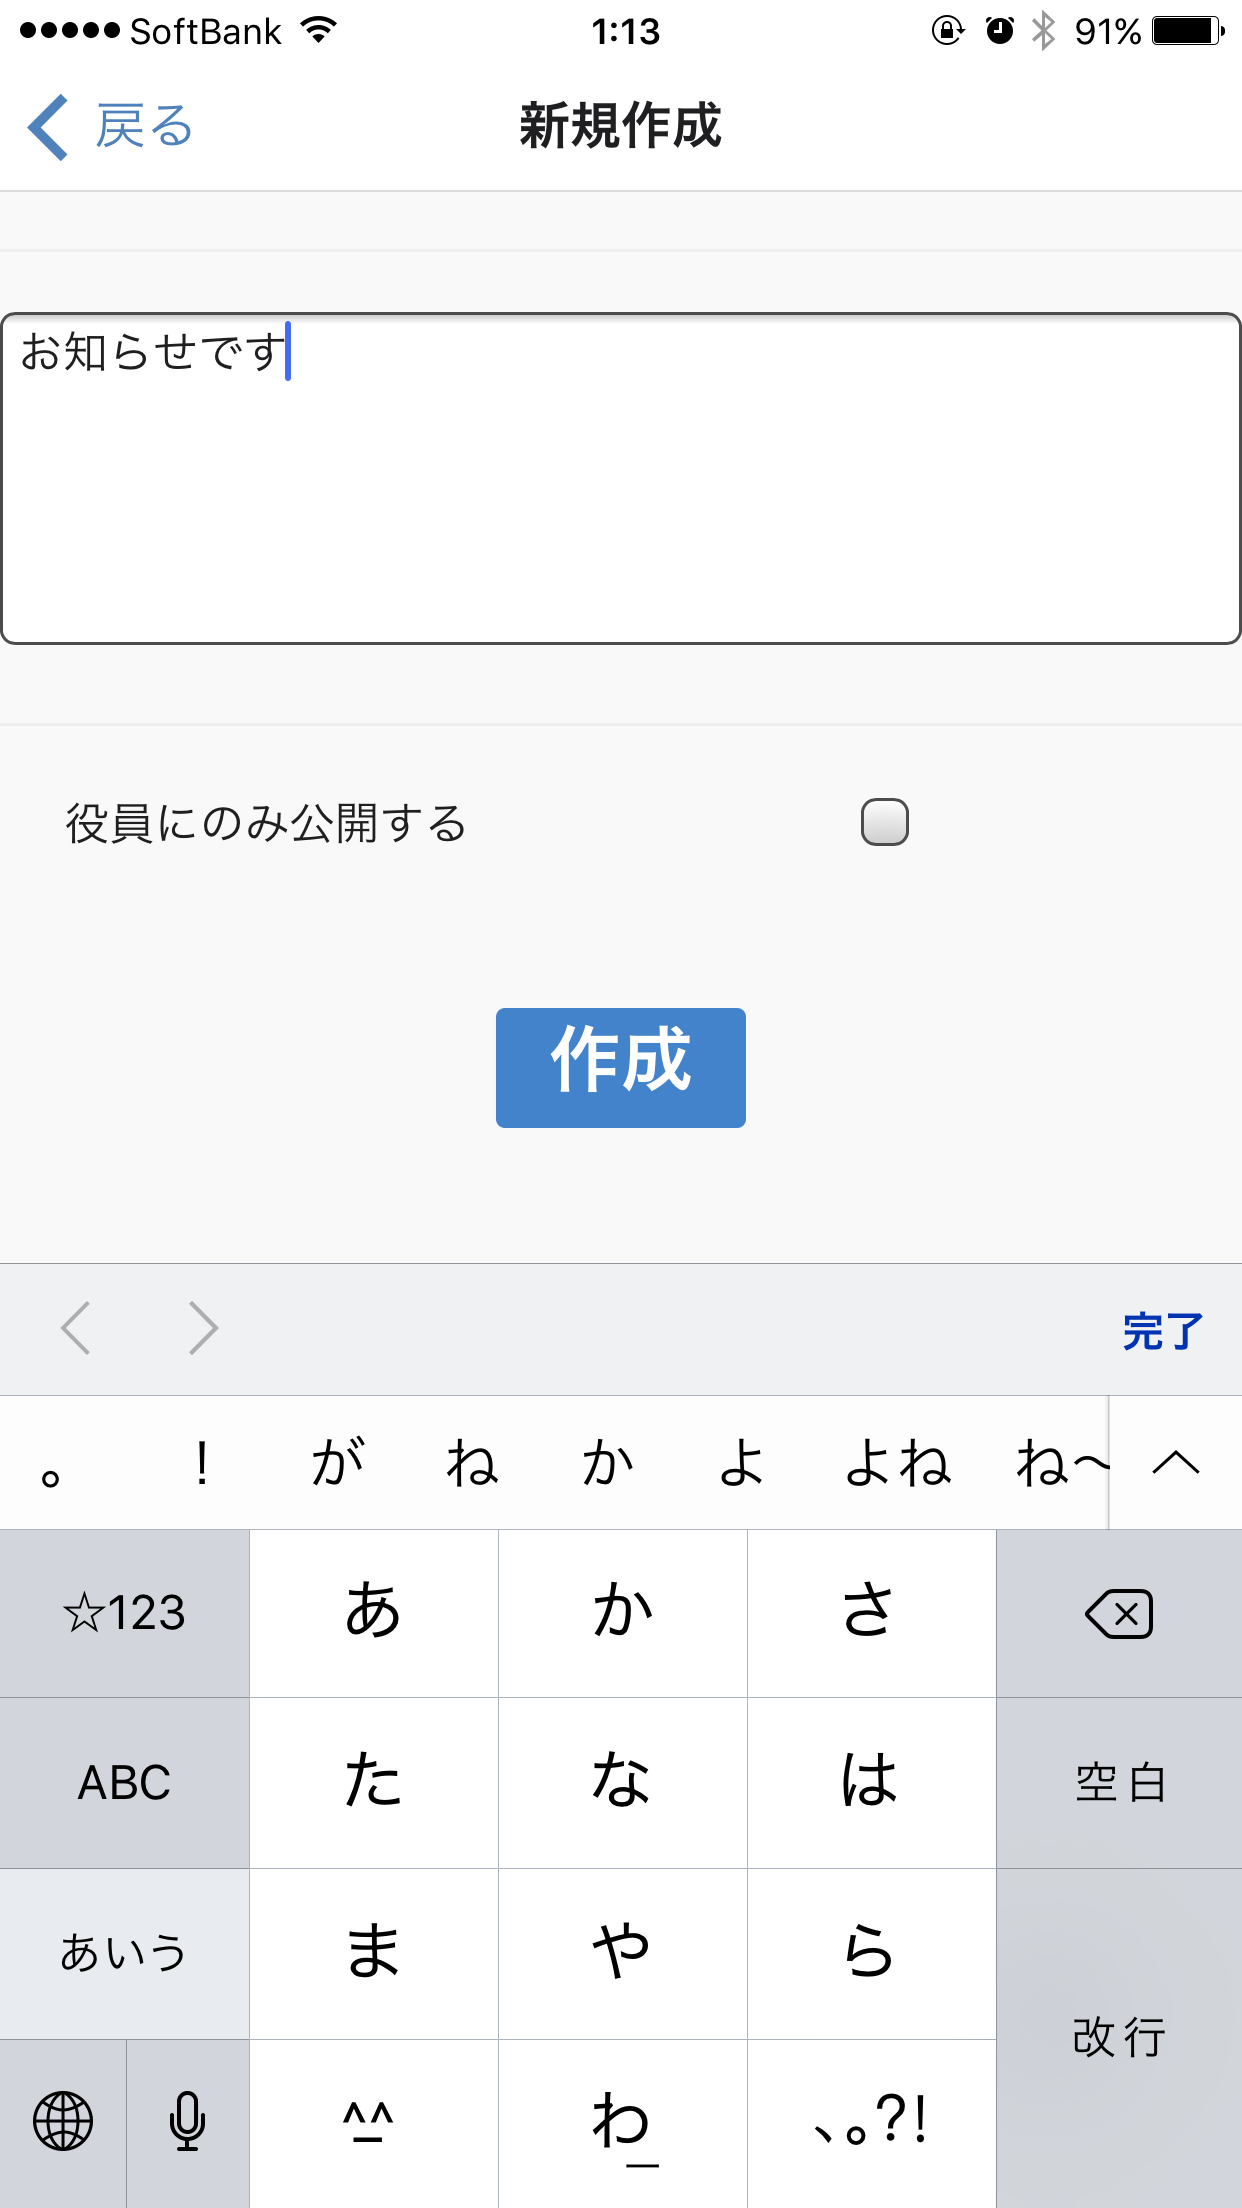
\includegraphics[width=4cm]{notification_add.PNG}
          \hspace{1cm}% (b)観光スポットの詳細情報
          {\footnotesize (b)削除を実行した画面}
        \end{center}
      \end{minipage}

    \end{tabular}
    \caption{お知らせ削除}
    \label{fig:lena}
  \end{center}
\end{figure}

\section{通知機能}%例:レビュー内容
通知機能とは、イベント管理の各機能及びお知らせが発信された際に本アプリケーションがインストールされている全ての端末に、各情報を通知する(図5.7)機能である。通知機能は、NCMBが提供するプッシュ通知機能を用いた。

\begin{figure}[htbp]
  \begin{center}
    \begin{tabular}{c}

      % 1
      \begin{minipage}{0.33\hsize}
        \begin{center}
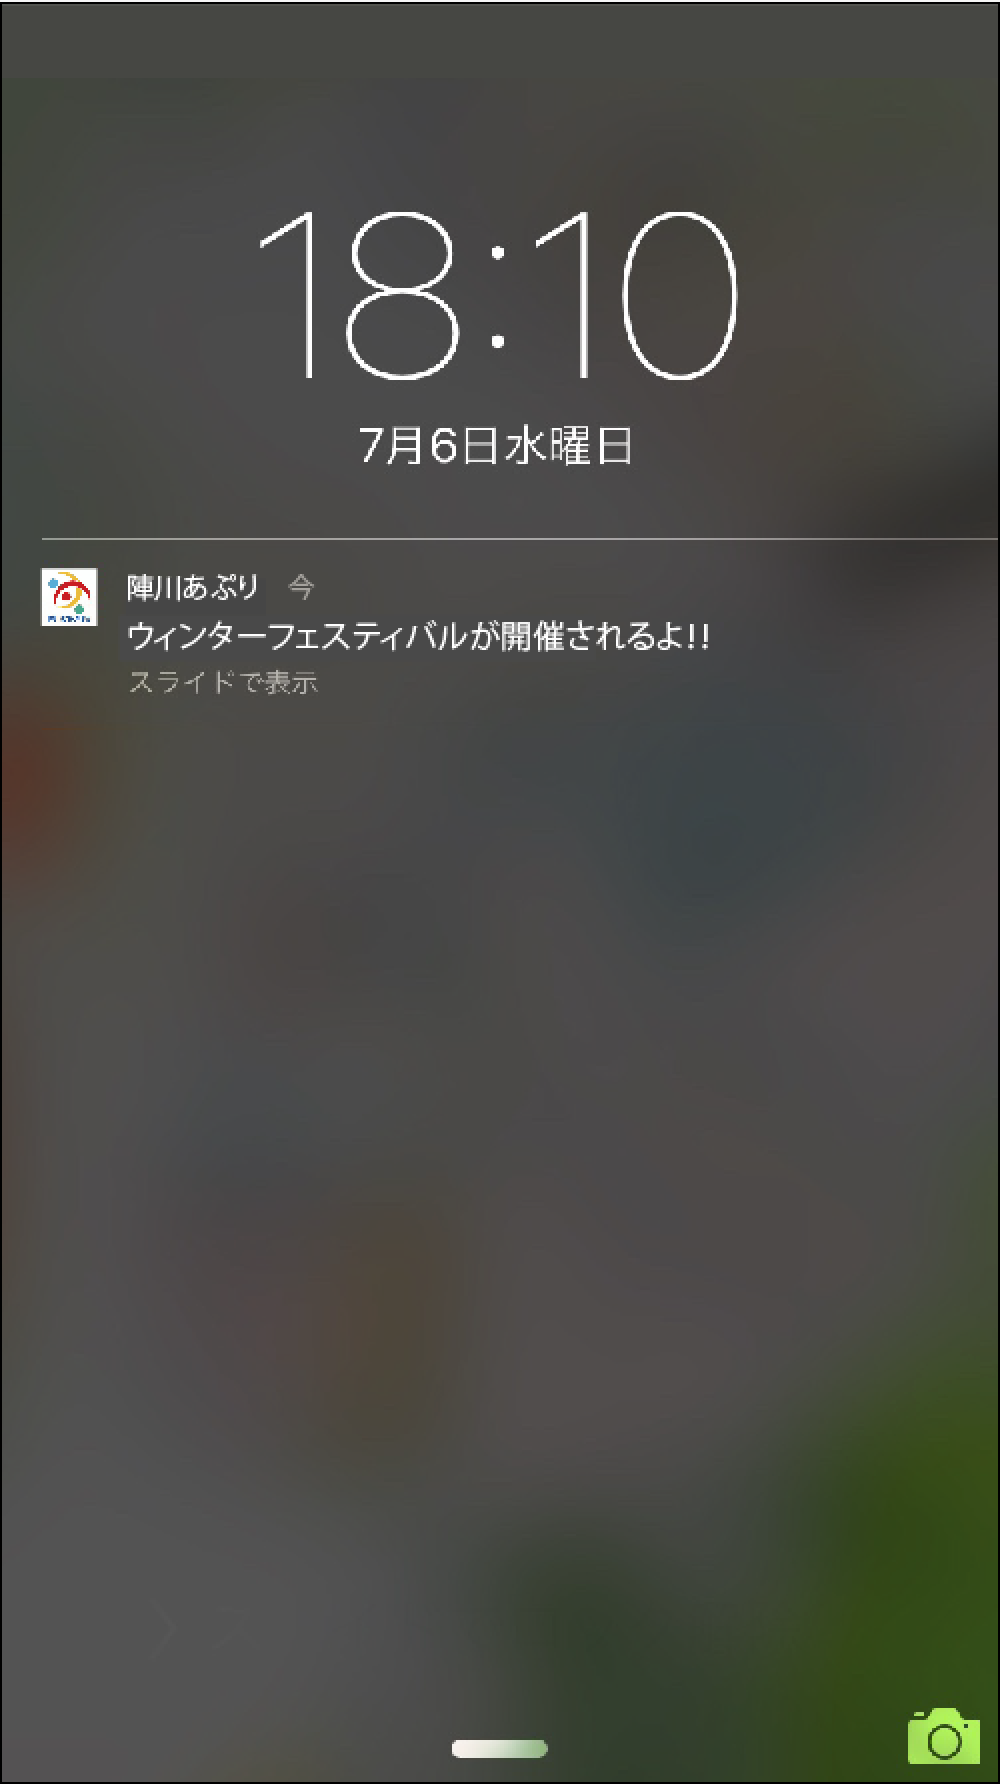
\includegraphics[width=4cm]{notification.png}
          \hspace{1cm} %(a)観光スポットの紹介
          {\footnotesize (a)通知イメージ}
        \end{center}
      \end{minipage}

    \end{tabular}
    \caption{通知機能}
    \label{fig:lena}
  \end{center}
\end{figure}

\bunseki{横山新}

